\chapter{Implementierung}\label{chap:implementierung}

Aufbauend auf der in Abschnitt~\ref{ssec:implementierungsidee} vorgeschlagenen Programmstruktur wird in diesem Kapitel
die Implementierung des \gls{fdk} mit der CUDA-Plattform beschrieben. Dazu werden zunächst die Grundlagen der
Programmierung mit CUDA erläutert, woran sich in den folgenden Abschnitten die konkrete Implementierung anschließt.

\section{Grundlagen der CUDA-Programmierung}\label{sec:grundlagen_cuda}

Als Basis für die in den nachfolgenden Abschnitten vorgestellte Implementierung dient die CUDA-Plattform der Firma
NVIDIA\@. Dieser Abschnitt stellt dieses technische Fundament anhand seiner historischen Entwicklung sowie der für diese
Arbeit wichtigen Konzepte vor.

\subsection{Programmierbare Grafikkarten}\label{ssec:cu_prog_gpu}

Als NVIDIA im Jahre 2006 seine \textit{Compute-Unified-Device-Architecture}-Plattform (CUDA) vorstellte, die die
direkte Programmierung der NVIDIA-Grafikkarten ermöglichte, folgte die Firma damit einer Entwicklung, die in den ersten
Jahren des neuen Jahrtausends begonnen hatte. Mit der Einführung der NVIDIA GeForce 3 im Jahre 2001 und der parallelen
Veröffentlichung von \gls{directx} 8 bzw.\ \gls{opengl} \textit{Vertex-Shader}-Erweiterungen hatten Anwendungsentwickler
erstmals Zugriff auf die \textit{Shader}-Einheiten für die \textit{Vertex}- und
\textit{Transform-\&-Lighting}-Berechnung. Spätere \gls{gpu}s, die mit \gls{directx} 9 kompatibel waren, gestatteten
eine noch flexiblere Programmierung, indem sie Entwicklern Zugriff auf die \textit{Pixel-Shader} erlaubten und die
Nutzung von Texturen im \textit{Vertex-Shader} zuließen. Die 2002 vorgestellte \gls{gpu} ATI Radeon 9700 verfügte über
einen programmierbaren 24bit-Fließkommazahl-\textit{Pixel-Shader}-Prozessor, der mit \gls{directx} 9 und \gls{opengl}
gesteuert werden konnte, die GeForce FX bot sogar 32bit-Fließkommazahl-Pixel-Prozessoren. Diese programmierbaren
Prozessoren waren Teil einer Entwicklung, die zu einer allmählichen Vereinheitlichung der auf der \gls{gpu} verbauten
Funktionseinheiten führte: während es auf den GeForce-Serien 6800 und 7800 noch getrennte Prozessoren für die
\textit{Vertex}- und \textit{Pixel}-Berechnung gab, wurde in der 2005 erschienenen XBox 360 eine
{\glqq}vereinheitlichte{\grqq} Grafikkarte verbaut, deren Prozessoreinheiten sowohl für die \textit{Vertex}- als auch
für die \textit{Pixel}-Berechnung geeignet waren. (vgl.~\cite{kirkhwu}, S. 28 -- 29)

Durch diese Vereinheitlichung der \gls{gpu}-Prozessoren glich die Hardware mehr und mehr den aus dem \gls{hpc} bekannten
Parallelrechnern. Mit der Verfügbarkeit \gls{directx}-9-kompatibler \gls{gpu}s wurde diese Entwicklung zunehmend
auch in Forschungskreisen bekannt und man begann zu untersuchen, inwiefern sich die neue Hardware zur Lösung von
berechnungsintensiven Problemen aus den Bereichen der Natur- und Ingenieurswissenschaften einsetzen ließ. Die zu diesen
Zwecken nicht konstruierten \gls{gpu}s ließen sich jedoch nur über die vorhandenen Schnittstellen zur
Grafikprogrammierung ansteuern. Zur Nutzung der Hardwareressourcen musste ein Programmierer daher das zu lösende Problem
zunächst auf computergrafische Operationen abbilden, sodass die Berechnung dann mit \gls{opengl} oder \gls{directx}
durchgeführt werden konnte. Um beispielsweise eine mathematische Funktion mehrfach auszuführen, musste diese erst in
ein \textit{Pixel-Shader}-Programm umgeschrieben werden, während die zugehörigen Eingabedaten als Texturen
vorzuliegen hatten und die Ausgabedaten im der jeweiligen Grafikbibliothek eigenen Pixelformat zurückgegeben wurden.
Die Umschreibung in einen für die Verwendung von \textit{Pixel-Shadern} geeigneten Algorithmus hatte außerdem den
gravierenden Nachteil, dass Zugriffe auf beliebige Stellen im Speicher nicht möglich waren. Da ein \textit{Pixel-Shader}
als Ausgabedatum die Farbe eines \gls{pixel}s zurückliefert, besteht dazu aus Sicht der Grafikbibliothek auch keine
Notwendigkeit, da die Position des zugehörigen Pixels bereits bekannt ist. (vgl.~\cite{kirkhwu}, S. 33)

Diese Beschränkungen erwiesen sich für generische numerische Berechnungen bald als zu restriktiv. Erschwerend kam hinzu, 
dass jeder Entwickler, der sich mit diesen technischen Limitierungen abfinden konnte, zusätzlich noch Wissen über die
Funktionsweise von \gls{opengl} und \gls{directx} benötigte, um das zu lösende Problem mit Hilfe von \gls{gpu}s
bewältigen zu lassen. Eine flächendeckende Akzeptanz von \gls{gpu}s als Beschleunigern war unter Forschern daher in den
ersten Jahren des \gls{gpgpu} nicht gegeben. (vgl.~\cite{sandkand}, S. 6)

Die Situation änderte sich, als NVIDIA 2006 die GeForce 8800 GTX der Öffentlichkeit präsentierte. Diese \gls{gpu} war
nicht nur zum damals neuen \gls{directx} 10 kompatibel, sondern auch die erste Grafikkarte, die mit \gls{cuda} ohne den
Umweg über \gls{directx} oder \gls{opengl} direkt programmierbar war (vgl.~\cite{sandkand}, S. 7). Programmierer hatten
nun die Möglichkeit, \textit{datenparallele} Aspekte (vgl. Abschnitt~\ref{cuda:modell}) des zu lösenden Problems zu
deklarieren und von der \gls{gpu} ausführen zu lassen. Die \textit{Shader}-Prozessoren hatten sich zu komplett
programmierbaren Prozessoren entwickelt und verfügten über einen Instruktionsspeicher, einen Instruktions-Cache und eine
Instruktionskontrollogik. Diesen zusätzlichen Hardwareoverhead konnte NVIDIA dadurch reduzieren, dass mehrere
Prozessoren sich den Instruktionscache und die -kontrolllogik teilten. Diese Struktur funktioniert aufgrund des
Hardware-Fokus auf die parallele Berechnung von \gls{pixel}n für \gls{gpu}s gut. Zusätzlich war es nun möglich, auf
beliebige Teile des Speichers zuzugreifen. Aus Sicht des Entwicklers lag nun ein Programmiermodell vor, das eine
Hierarchie paralleler Threads, Synchronisierungsmechanismen und Barrieren sowie atomare Operationen bot und das Ganze in
eine an C bzw.\ C++ angelehnte Sprache einbettete. (vgl.~\cite{kirkhwu}, S. 35)

\subsection{Das CUDA-Programmiermodell}\label{cuda:modell}

In diesem Abschnitt wird das der \gls{cuda}-Plattform zugrundeliegende Programmiermodell näher vorgestellt. Das
gedankliche Fundament dieses Modell ist die \textit{Datenparallelität}, die im Folgenden erläutert wird. Die konkreten
Programmierkonzepte schließen sich in den danach folgenden Abschnitten an.

\subsubsection*{Datenparallelität}

Moderne Programme bearbeiten häufig große Datenmengen und benötigen deswegen auf herkömmlichen Rechnern lange
Ausführungszeiten. Viele Anwendungen arbeiten dabei mit Daten, die Vorgänge der echten Welt ab- oder nachbilden, wie
beispielsweise einfache Bilder oder Filme oder die Bewegungen von Flüssigkeiten und Gasen unter bestimmten Umständen.
Fluglinien müssen ihre Flüge planen, wozu die Daten einer Vielzahl anderer Flüge, Besatzungen und Flughäfen herangezogen
werden, die voneinander unabhängig sind. Diese Unabhängigkeit der Daten ist die Voraussetzung für datenparallele
Algorithmen.

Als einfaches Beispiel für einen datenparallelen Algorithmus lässt sich die Addition zweier Vektoren $A$ und $B$
betrachten:

\begin{equation*}
    \left(
        \begin{array}{c}
            a_1\\
            a_2\\
            a_3
        \end{array}
    \right)
    +
    \left(
        \begin{array}{c}
            b_1\\
            b_2\\
            b_3
        \end{array}
    \right)
    =
    \left(
        \begin{array}{c}
            a_1 + b_1 \\
            a_2 + b_2 \\
            a_3 + b_3
        \end{array}
    \right)
    =
    \left(
        \begin{array}{c}
            c_1 \\
            c_2 \\
            c_3
        \end{array}
    \right)
\end{equation*}

In diesem Beispiel wird $c_1$ berechnet, indem $a_1$ und $b_1$ addiert werden, und $c_3$ ergibt sich aus der Addition
von $a_3$ und $b_3$. Die Additionen sind voneinander unabhängig und können parallel berechnet werden. Sehr große
Vektoren führen in diesem Beispiel daher zu einem hohen Maß an Datenparallelität.

Der Datenparallelität steht das Konzept der \textit{Task-Parallelität} gegenüber. Die Task-Parallelität kommt vor allem
in komplexeren Programmen zur Anwendung, in denen es mehrere unterschiedliche Aufgaben gibt, die parallel bearbeitet
werden können. Vorstellbar ist z.B.\ ein Programm zur Filterung von Bildern, in denen ein Task die Bilder nacheinander
lädt, der zweite die Bilder nacheinander filtert und ein weiterer die gefilterten Bilder wieder abspeichert.
(vgl.~\cite{kirkhwu}, S. 42 -- 43)

\subsubsection*{Parallele Ausführung}

Die Ausführung eines \gls{cuda}-Programms beginnt auf dem \gls{host}. Wird ein \gls{kernel} aufgerufen, so wird auf dem
\gls{device} eine Anzahl an Threads gestartet. Die Summe aller auf dem \gls{device} gestarteten Threads bezeichnet
man als \textit{\gls{grid}}. Haben alle Threads eines \gls{kernel}s ihre Ausführung beendet, wird auch das \gls{grid}
beendet. Das Starten eines \gls{kernel}s erzeugt typischerweise eine große Zahl von Threads. Im Gegensatz zur \gls{cpu},
auf der das Erzeugen eines Threads in der Regel mehrere tausend Zyklen benötigt, ist der gleiche Vorgang auf der
\gls{gpu} in einigen wenigen Zyklen zu bewältigen. (vgl.~\cite{kirkhwu}, S. 44 -- 45)

Das oben vorgestellte Beispiel der Vektoraddition lässt sich in C++, wie in Quelltext~\ref{source:vec_add_cpp}
dargestellt, durch die Iteration über die Vektoren implementieren.  In \gls{cuda} entfällt die Iteration, da hier 
jeder Thread ein Element des Ausgabevektors $C$ berechnet, wie in Quelltext~\ref{source:vec_add_cuda} gezeigt.

\begin{listing}
\begin{minted}[breaklines,breakafter=\,,fontsize=\small]{c++}
auto vec_add(const std::int32_t* A, const std::int32_t* B,
             std::int32_t* C, std::size_t size) -> void
{
    for(auto i = 0u; i < size; ++i)
        C[i] = A[i] + B[i];
}
\end{minted}
\caption{Vektoraddition mit C++}
\label{source:vec_add_cpp}
\end{listing}

\begin{listing}
\begin{minted}[breaklines,breakafter=\,,fontsize=\small]{cuda}
__global__ void vec_add(const std::int32_t* A, const std::int32_t* B,
                        std::int32_t* C, std::size_t size)
{
    auto i = blockIdx.x * blockDim.x + threadIdx.x;
    if(i < size)
        C[i] = A[i] + B[i];
}
\end{minted}
\caption{Vektoraddition mit \gls{cuda}}
\label{source:vec_add_cuda}
\end{listing}

Die Berechnung der Indices erfolgt in diesem Beispiel nicht über eine fortlaufend inkrementierte Variable, wie es in C++
der Fall wäre, sondern über die Hilfsvariablen \texttt{blockIdx}, \texttt{blockDim} und \texttt{threadIdx}. Wird ein
\gls{cuda}-\gls{kernel} ausgeführt, so entsteht auf dem \gls{device} ein Thread-\gls{grid}. Diese Threads werden in
einer zweistufigen Hierarchie angeordnet. Jedes \gls{grid} besteht aus mehreren Thread-Blöcken, die der Einfachheit
halber in der Folge als \textit{Blöcke} bezeichnet werden. Alle Blöcke innerhalb eines \gls{grid}s haben die gleiche
Größe, können jedoch auf aktueller Hardware maximal 1024 Threads umfassen; die Thread-Zahl der Blöcke wird auf dem
\gls{host} vor der Ausführung des \gls{kernel}s definiert. Für ein gegebenes \gls{grid} kann die Anzahl der Threads pro
Block durch die Variable \texttt{blockDim} abgefragt werden, während der individuelle Block, zu dem ein bestimmter
Thread gehört, durch die Variable \texttt{blockIdx} identifiziert werden kann. Innerhalb eines Blocks kann ein einzelner
Thread über die ariable \texttt{threadIdx} bestimmt werden. Durch die Kombination der drei Variablen, wie sie in
Quelltext~\ref{source:vec_add_cuda} dargestellt ist, lässt sich somit jeder Thread innerhalb des \gls{grid}s eindeutig
identifizieren. Da \gls{cuda} das Starten von zwei- und dreidimensionalen \gls{kernel}n unterstützt, kann über die
Felder \texttt{x}, \texttt{y} und \texttt{z} die Zahl der Blöcke bzw.\ Threads in der jeweiligen Dimension bestimmt
werden. (vgl.~\cite{kirkhwu}, S. 54)

Ein weiterer Unterschied zur herkömmlichen C++-Programmierung ist das Schlüsselwort \texttt{\_\_global\_\_} vor der
Deklaration. Dieses Schlüsselwort dient zur Identifizierung einer Funktion als \gls{kernel}, also einer Funktion auf
dem \gls{device}, die vom \gls{host} aus aufgerufen werden kann. Daneben verwendet \gls{cuda} die Schlüsselworte
\texttt{\_\_device\_\_} und \texttt{\_\_host\_\_}, die anzeigen, auf welcher Hardware die jeweilige Funktion ausgeführt
werden kann bzw.\ soll. Eine \texttt{\_\_device\_\_}-Funktion kann dabei nur innerhalb eines \gls{kernel}s oder einer
weiteren \texttt{\_\_device\_\_}-Funktion aufgerufen werden, eine \texttt{\_\_host\_\_}-Funktion nur auf dem \gls{host}
-- sie entspricht also einer normalen C++-Funktion (siehe Tabelle~\ref{table:cu_func_keywords}). (vgl.~\cite{kirkhwu},
S. 55)

\begin{table}
    \centering
    \begin{tabular}{| l | c | c |}
        \hline
        & Ausgeführt auf dem & Aufgerufen vom \\
        \hline
        \texttt{\_\_device\_\_ float device\_func()} & \gls{device} & \gls{device} \\
        \hline
        \texttt{\_\_global\_\_ void kernel\_func()} & \gls{device} & \gls{host} \\
        \hline
        \texttt{\_\_host\_\_ float host\_func()} & \gls{host} & \gls{host} \\
        \hline
    \end{tabular}
    \caption{\gls{cuda}-Schlüsselworte für die Funktionsdeklaration}
    \label{table:cu_func_keywords}
\end{table}

\subsubsection*{Architektur}

Wird ein \gls{grid} auf dem \gls{device} zur Ausführung gebracht, werden ihm die Hardware-Ressourcen blockweise
zugeordnet. In der gegenwärtigen Hardware-Generation werden diese Ressourcen in \gls{sm}-Einheiten organisiert, auf
denen die Blöcke dann ausgeführt werden. Jeder \gls{sm} kann nur eine begrenzte Zahl von Blöcken gleichzeitig ausführen,
die durch zu wenige Ressourcen für den konkreten \gls{kernel} weiter reduziert werden kann. Wenn ein \gls{device}
beispielsweise bis zu 32 Blöcke pro \gls{sm} parallel ausführen kann, für die Threads aber nicht genügend Ressourcen
vorhanden sind, so wird die Zahl der parallel ausgeführten Blöcke automatisch verringert, bis ihr gemeinsamer
Ressourcenbedarf vom \gls{sm} bedient werden kann. Die meisten Grids bestehen aus mehr Blöcken, als gleichzeitig auf dem
\gls{device} ausgeführt werden können. Die CUDA-Laufzeitumgebung verwaltet die inaktiven Blöcke in einer Liste und
ordnet sie \gls{sm}s zu, sobald diese die Ausführung eines vorherigen Blocks abgeschlossen haben. (vgl.~\cite{kirkhwu},
S. 84)

Eine der Ressourcen, die einem \gls{sm} zugeordnet werden, ist die Zahl der Threads, die parallel verwaltet
werden kann. Diese Verwaltung benötigt wiederum Hardware-Ressourcen, um beispielsweise die Thread- und Block-Indices
speichern zu können. Gegenwärtige CUDA-fähige \gls{gpu}s können jedem \gls{sm} bis zu 2048 Threads zuordnen, z.B. in der
Form von vier Blöcken mit je 512 Threads, acht Blöcken mit je 256 Threads, etc. Besteht ein \gls{device} aus 20
\gls{sm}s und kann jeder dieser \gls{sm}s bis zu 2048 Threads verwalten, kann das \gls{device} insgesamt bis zu 40.960
Threads parallel ausführen. (vgl.~\cite{kirkhwu}, S. 84 -- 85)

\subsubsection*{Speicher}

Wie auf einem klassischen Rechner mit seinem Hauptspeicher, diversen Caches und Prozessorregistern gibt es auch auf
einer \gls{cuda}-fähigen \gls{gpu} verschiedene Möglichkeiten zur Zwischenspeicherung von Daten. Vom \gls{host} aus
können Daten entweder in den globalen Speicher (\textit{global memory}) oder in den konstanten Speicher
(\textit{constant memory}) kopiert werden. Wie der Name bereits andeutet, kann das \gls{device} nur lesend auf den
konstanten Speicher zugreifen. Dessen Vorteil gegenüber dem globalen Speicher liegt in Speicherzugriffen mit geringerer
Latenz und höherer Bandbreite sowie speziellen Caches, er ist jedoch auf allen aktuellen \gls{gpu}s auf 64 KiB
beschränkt. Ähnlich wie der Hauptspeicher der \gls{cpu} ist dieser Speicher in Form von speziellen RAM-Modulen auf dem
\gls{device} verbaut und mit dem Chip über ein Bus-System verbunden (\textit{off-chip}). (vgl.~\cite{kirkhwu}, S. 101)

Direkt auf dem Chip (\textit{on-chip}) befinden sich die Register und der geteilte Speicher (\textit{shared memory}),
auf die die Threads mit hoher Geschwindigkeit zugreifen können. Register werden einem Thread fest zugeordnet und können
nur von diesem gelesen und beschrieben werden, ein Zugriff auf die Register anderer Threads ist nicht möglich. In einem
Register werden beispielsweise häufig verwendete, aber lokale Variablen zwischengespeichert. Der geteilte Speicher steht
einem ganzen Block zur Verfügung; alle Threads innerhalb desselben Blocks können auf diesen Speicher zugreifen, was dem
schnellen Datenaustausch dient. Sowohl die Register als auch der geteilte Speicher werden von einem \gls{sm} verwaltet
und können bei einem zu hohen Bedarf pro Thread bzw.\ Block die Zahl der parallel ausgeführten Blöcke verringern.
(vgl.~\cite{kirkhwu}, S. 101 -- 102)

Neben den Registern gibt es einen weiteren Speichertyp, der individuellen Threads zugeordnet werden kann, den lokalen
Speicher (\textit{local memory}). Dieser wird vom Compiler unter anderem automatisch dann einem \gls{kernel} zugewiesen,
wenn ein Thread ein privates Array anlegt oder wenn der Thread mehr Register benötigt, als vorhanden sind. De facto
handelt es sich beim lokalen Speicher um einen Teil des globalen Speichers, der sich aus Sicht des \gls{kernel}s wie ein
Register verhält. Da er sich nicht \textit{on-chip} befindet, ist der Zugriff auf ihn aber wesentlich langsamer und
deshalb in den meisten Anwendungsfällen nicht wünschenswert. (vgl.~\cite{kirkhwu}, S. 103)

Für den lesenden Zugriff auf den globalen Speicher gibt es zusätzlich den Texturspeicher. Obwohl dieser eigentlich für
den Einsatz im Rahmen von \gls{opengl} und \gls{directx} konzipiert wurde, verfügt er über einige Funktionen, die seine
Verwendung in allgemeinen Berechnungen rechtfertigen. Wie der konstante Speicher verfügt auch der Texturspeicher über
spezielle Caches auf dem Chip, die wiederholte Zugriffe auf den \textit{off-chip}-befindlichen globalen Speicher
reduzieren. Diese Caches sind insbesondere dann nützlich, wenn die Speicherzugriffe auf örtlich zusammenhängende
Datenbereiche erfolgen, wie etwa benachbarte \gls{pixel} eines Bildes. Da Texturen auch zwei- oder dreidimensional
sein können, ist das Caching der benachbarten Pixel besonders interessant, da vertikal benachbarte Pixel in einem
Speicherbereich normalerweise weit auseinander liegen und somit selten gemeinsam in herkömmlichen Caches liegen.
Zusätzlich verfügt der Texturspeicher über spezielle Maschinenbefehle für die Pixelinterpolation (\textit{nearest
neighbour} und linear). (vgl.~\cite{sandkand}, S. 116 -- 117)

Neben Texturen besitzt CUDA einen weiteren Mechanismus, um effizient auf mehrdimensionale Speicherbereiche zuzugreifen,
den sogenannten \textit{pitched memory}. Durch das Einfügen zusätzlicher Bytes am Ende einer Zeile kann der Speicher
anhand der Wortbreite (zur Zeit entweder 32, 64 oder 128 Byte) so ausgerichtet werden, dass jede neue Zeile am Anfang
eines neuen Speicherwortes steht. Ist eine Zeile beispielsweise 16 Byte lang, aber über zwei Speicherworte verteilt,
muss zweimal auf den Speicher zugegriffen werden, um sie komplett auszulesen. Platziert man den Zeilenanfang jedoch am
Anfang eines Speicherwortes, genügt ein Zugriff. Der Speicherzugriff wird also effizienter, geht jedoch mit einem
insgesamt erhöhten Speicherbedarf einher. (vgl.~\cite{cudaprog}, Abschnitt 5.3)

Die verschiedenen Speichervarianten sind in Tabelle~\ref{table:cu_mem_hierarchie} zusammengefasst.

\begin{table}
    \centering
    \begin{tabular}{| l | c | c | c |}
        \hline
        Bezeichnung & Ort & Sichtbarkeit & Zugriff\\
        \hline
        \hline
        Register & On-Chip & pro Thread & lesen / schreiben \\
        \hline
        \texttt{\_\_shared\_\_} & On-Chip & pro Block & lesen / schreiben \\
        \hline
        \texttt{\_\_global\_\_} & Off-Chip & pro Kernel & lesen / schreiben \\
        \hline
        \texttt{\_\_constant\_\_} & Off-Chip & pro Kernel & nur lesen \\
        \hline
        \texttt{\_\_local\_\_} & Off-Chip & pro Thread & lesen / schreiben\\
        \hline
        Textur & Off-Chip & pro Kernel & nur lesen\\
        \hline
    \end{tabular}
    \caption{Die verschiedenen Varianten des \gls{cuda}-Speichers}
    \label{table:cu_mem_hierarchie}
\end{table}

\subsubsection*{Streams}

Grundsätzlich werden alle Operationen auf der GPU in der Reihenfolge ihrer Aufrufe ausgeführt. Um Aufgaben parallel
ausführen zu können, gibt es die Möglichkeit, weitere Warteschlangen auf dem \gls{device} anzulegen und diesen
Operationen zuzuordnen. Auf der \gls{cuda}-Plattform werden diese Warteschlangen \glspl{stream} genannt. Innerhalb eines
\glspl{stream} werden die zugehörigen Anweisungen wieder in der Reihenfolge ihres Aufrufs ausgeführt, jedoch unabhängig
von den Aufgaben anderer \glspl{stream} und -- die nötigen Hardwareressourcen vorausgesetzt -- zu diesen parallel. Im
Kontext dieser Arbeit ist vor allem interessant, dass Datenkopien vom \gls{host} zum \gls{device} und umgekehrt
ebenfalls in einem \gls{stream} ablaufen können, sodass sie parallel zu der Ausführung eines \gls{kernel}s durchgeführt
werden. Die für die Kopie benötigte Zeit kann somit durch die parallel stattfindenden Berechnungen versteckt werden und
fällt für die Gesamtlaufzeit des Algorithmus nicht mehr ins Gewicht, sofern die Berechnungen länger dauern.
(vgl.~\cite{sandkand}, S. 198f.)

\section{Optimierungsziele}\label{optimierungsziele}

Die Rückprojektion erfordert im Vergleich zur Wichtung und Filterung einen weitaus höheren Rechenaufwand. Ihrer
Optimierung ist deshalb die höchste Priorität einzuräumen, sodass der gesamte Algorithmus für derzeit gängige Datensätze
der Computertomographie -- also bis zu einer Projektionsauflösung von 1024 $\times$ 1024 \gls{pixel}n -- auf neuer
Hardware in wenigen Minuten lösbar ist. Da die \gls{cuda}-Plattform den parallelen Einsatz mehrerer \gls{gpu}s
unterstützt, ist die Implementierung so zu konzipieren, dass sie auf einer oder mehreren Grafikkarten lauffähig ist.

\subsection*{Vorüberlegungen}

Weil die gefilterte Rückprojektion von einer Reihe geometrischer Parameter abhängt, ist die Zahl der benötigten Register
für die Übergabe dieser Parameter sowie zur Speicherung von Zwischenergebnissen recht hoch. Ein großer Teil dieser
Parameter ist jedoch während der Rückprojektion konstant, wie zum Beispiel die Abstände zwischen dem Objekt, der Quelle
und dem Detektor oder die geometrischen Eigenschaften des Detektors. Es empfiehlt sich daher, diese in den konstanten
Speicher der Grafikkarte auszulagern, um den Bedarf an den zwischen den Threads geteilten Ressourcen zu minimieren und
dadurch die potentielle Auslastung zu erhöhen.

Anders verhält es sich mit den Projektionen und dem Volumen. Weil während der Ausführung auf beide Speicherbereiche
schreibend zugegriffen werden muss, ist es sinnvoll, diese Zugriffe möglichst optimal zu gestalten. Da die Projektionen
der Kegelstrahltomographie zweidimensional sind und das zu rekonstruierende Volumen dreidimensional ist, können die für
zwei- bzw.\ dreidimensionale Operationen optimierten Speichervarianten der \gls{cuda}-Plattform verwendet werden, die in
Abschnitt~\ref{cuda:modell} vorgestellt wurden. Zusätzlich ist es nach der Wichtung und der Filterung nicht mehr
erforderlich, die Projektionen zu verändern. Durch deren Umwandlung in Texturen bzw.\ deren Verschiebung in den für
Texturzugriffe optimierten Teil des globalen Speichers, kann während der Rückprojektion der Zeitbedarf für den Zugriff
auf die Projektionen minimiert werden.

\section{Geometriebeschreibung}

Die in Kapitel~\ref{grundlagen_bp} vorgestellten theoretischen Methoden zur Berechnung der Rückprojektion bedürfen vor
ihrer Implementierung noch einiger geometrischer Anpassungen bzw.\ Erweiterungen, um einigen in der Praxis auftretenden
Hürden gerecht zu werden. Diese werden in den folgenden Abschnitten vorgestellt.

\subsection{Detektorgeometrie}

Der Detektor übt aufgrund der durch ihn gewonnenen Informationen (in Form der Projektionen) einen großen Einfluss auf
die gefilterte Rückprojektion aus. Seinem Aufbau muss daher bei der Implementierung des \gls{fdk} besondere
Aufmerksamkeit zukommen.

Der Detektor hat eine feste Breite und Höhe (gemessen in Millimetern) und besteht aus einer zweidimensionalen Anordnung
von \gls{pixel}n (siehe Abbildung~\ref{fig:det_geometrie}). In der horizontalen Richtung verfügt er über $N_h$
\gls{pixel}, in der vertikalen Richtung sind es $N_v$ \gls{pixel}.

Jedes \gls{pixel} hat eine physische Breite $d_h$ und Höhe $d_v$ (gemessen in Millimetern); äquivalent lassen sich diese
Ausdehnungen als horizontale (vertikale) Abstände zwischen den \gls{pixel}zentren betrachten (siehe
Abbildung~\ref{fig:det_pixel}).

Spannt man nun über dem Detektor ein Koordinatensystem auf (mit dessen Zentrum als Ursprung, siehe
Abbildung~\ref{fig:det_koord}), wobei $h_{min}$, $h_{max}$, $v_{min}$ und $v_{max}$ den horizontalen (vertikalen)
Abstand von den Detektorrändern bis zur Detektormitte in Millimetern angeben, so ergeben sich die folgenden
Zusammenhänge:

\begin{equation}\label{eq:det_h}
    \begin{aligned}
        h_{max} - h_{min} &= N_h \cdot d_h\\
        h_{min} + \frac{N_h \cdot d_h}{2} &= 0
    \end{aligned}
\end{equation}

\begin{equation}\label{eq:det_v}
    \begin{aligned}
        v_{max} - v_{min} &= N_v \cdot d_v\\
        v_{min} + \frac{N_v \cdot d_v}{2} &= 0
    \end{aligned}
\end{equation}

\begin{figure}[!tb]
    \centering
    \begin{minipage}[b]{.5\textwidth}
        \centering
        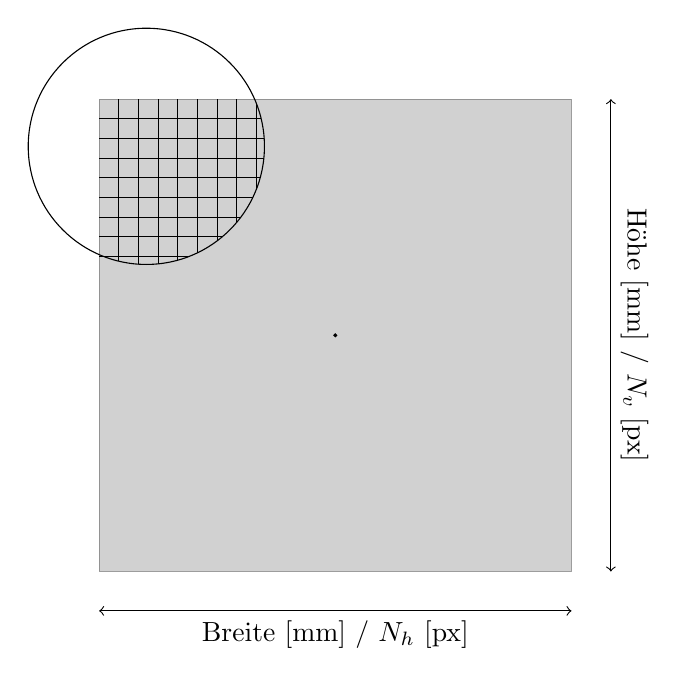
\begin{tikzpicture}
            \draw[fill=black!60!white,opacity=0.3] (-3, 3) -- (3, 3) -- (3, -3) -- (-3, -3) -- (-3, 3);
            \draw[fill=black] (0,0) circle (0.5pt);

            % Lupe
            \draw (-2.4, 2.4) circle (1.5cm);

            % Pixellinien vertikal
            \draw (-2.75, 3) -- (-2.75, 0.95);
            \draw (-2.5, 3) -- (-2.5, 0.9);
            \draw (-2.25, 3) -- (-2.25, 0.9);
            \draw (-2, 3) -- (-2, 0.95);
            \draw (-1.75, 3) -- (-1.75, 1.05);
            \draw (-1.5, 3) -- (-1.5, 1.2);
            \draw (-1.25, 3) -- (-1.25, 1.43);
            \draw (-1, 2.94) -- (-1, 1.85);

            % Pixellinien horizontal
            \draw (-3, 2.75) -- (-0.95, 2.75);
            \draw (-3, 2.5) -- (-0.9, 2.5);
            \draw (-3, 2.25) -- (-0.9, 2.25);
            \draw (-3, 2) -- (-0.95, 2);
            \draw (-3, 1.75) -- (-1.05, 1.75);
            \draw (-3, 1.5) -- (-1.2, 1.5);
            \draw (-3, 1.25) -- (-1.43, 1.25);
            \draw (-3, 1) -- (-1.85, 1);

            % Pfeile und Beschriftungen
            \draw[<->] (-3, -3.5) -- (3, -3.5) node[pos=0.5, below] {Breite [mm] / $N_h$ [px]};
            \draw[<->] (3.5, 3) -- (3.5, -3) node[pos=0.5, sloped, above] {Höhe [mm] / $N_v$ [px]};
        \end{tikzpicture}
        \captionof{figure}{Detektorgeometrie}
        \label{fig:det_geometrie}
    \end{minipage}%
    \begin{minipage}[b]{.5\textwidth}
        \centering
        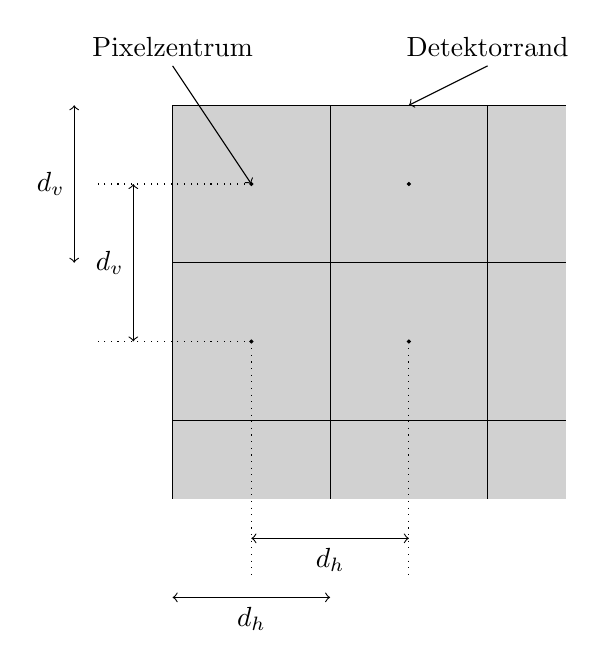
\begin{tikzpicture}
            \fill[black!60!white,opacity=0.3] (-2, 2) rectangle (3, -3);
            \draw (-2, 2) -- (2, 2) -- (2, -2) -- (-2, -2) -- (-2, 2);
            \draw (2, 2) -- (3, 2);
            \draw (-2, 0) -- (3, 0);
            \draw (0, 2) -- (0, -3);
            \draw (-2, 2) -- (-2, -3);
            \draw (2, -2) -- (2, -3);
            \draw (2, -2) -- (3, -2);
            \draw[fill=black] (-1, 1) circle (0.5pt);
            \draw[fill=black] (1, 1) circle (0.5pt);
            \draw[fill=black] (1, -1) circle (0.5pt);
            \draw[fill=black] (-1, -1) circle (0.5pt);

            % Verlängerungen
            \draw[dotted] (-1, 1) -- (-3, 1);
            \draw[dotted] (-1, -1) -- (-3, -1);
            \draw[dotted] (-1, -1) -- (-1, -4);
            \draw[dotted] (1, -1) -- (1, -4);

            % Pfeile und Beschriftungen
            \draw[->] (2, 2.5) -- (1, 2) node[pos=0, above] {Detektorrand};
            \draw[->] (-2, 2.5) -- (-1, 1) node[pos=0, above] {Pixelzentrum};
            \draw[<->] (-2.5, 1) -- (-2.5, -1) node[pos=0.5, left] {$d_v$};
            \draw[<->] (-3.25, 2) -- (-3.25, 0) node[pos=0.5, left] {$d_v$};
            \draw[<->] (-1, -3.5) -- (1, -3.5) node[pos=0.5, below] {$d_h$};
            \draw[<->] (-2, -4.25) -- (0, -4.25) node[pos=0.5, below] {$d_h$};
        \end{tikzpicture}
        \captionof{figure}{Pixelgeometrie}
        \label{fig:det_pixel}
    \end{minipage}
\end{figure}

\begin{figure}[!tb]
    \centering
    \begin{minipage}[b]{.5\textwidth}
        \centering
        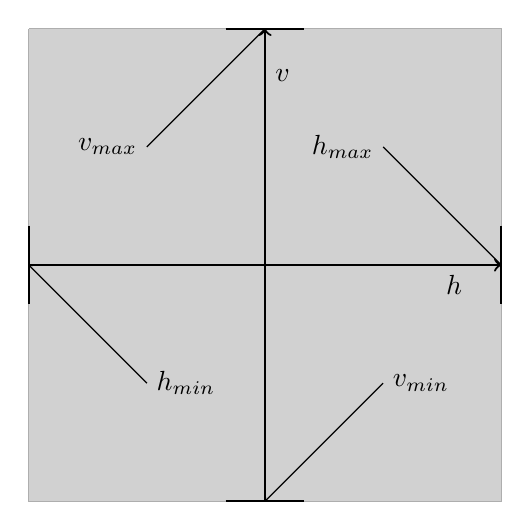
\begin{tikzpicture}[axis/.style={thick,->}]
            \draw[fill=black!60!white,opacity=0.3] (-3, 3) -- (3, 3) -- (3, -3) -- (-3, -3) -- (-3, 3);
            \draw[fill=black] (0,0) circle (0.5pt);

            % Achsen
            \draw[axis] (0, -3) -- (0, 3) node [pos=0.9, right] {$v$};
            \draw[axis] (-3, 0) -- (3, 0) node [pos=0.9, below] {$h$};

            % Markierungen
            \draw[thick] (-3, 0.5) -- (-3, -0.5);
            \draw[thick] (3, 0.5) -- (3, -0.5);
            \draw[thick] (-0.5, 3) -- (0.5, 3);
            \draw[thick] (-0.5, -3) -- (0.5, -3);

            % Beschriftungen
            \draw[->] (1.5, 1.5) -- (3, 0) node [pos=0, left] {$h_{max}$};
            \draw[->] (-1.5, -1.5) -- (-3, 0) node [pos=0, right] {$h_{min}$};
            \draw[->] (-1.5, 1.5) -- (0, 3) node [pos=0, left] {$v_{max}$};
            \draw[->] (1.5, -1.5) -- (0, -3) node [pos=0, right] {$v_{min}$};
        \end{tikzpicture}
        \caption{Detektorkoordinatensystem}
        \label{fig:det_koord}
    \end{minipage}%
    \begin{minipage}[b]{.5\textwidth}
        \centering
        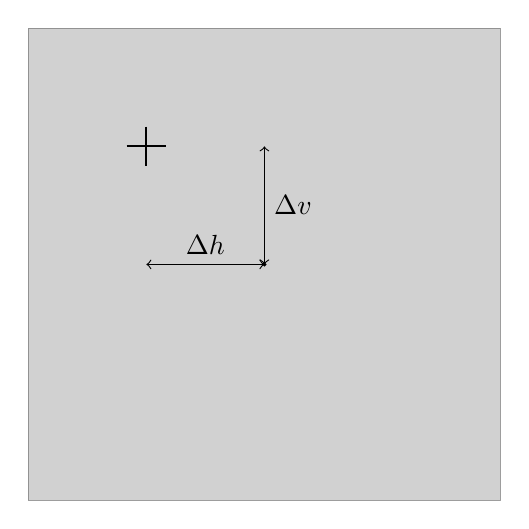
\begin{tikzpicture}
            \draw[fill=black!60!white,opacity=0.3] (-3, 3) -- (3, 3) -- (3, -3) -- (-3, -3) -- (-3, 3);
            \draw[fill=black] (0,0) circle (0.5pt);

            % Verschiebung
            \draw[thick] (-1.75, 1.5) -- (-1.25, 1.5);
            \draw[thick] (-1.5, 1.75) -- (-1.5, 1.25);

            % Pfeile & Beschriftung
            \draw[<->] (0, 1.5) -- (0, 0) node[pos=0.5,right] {$\Delta v$};
            \draw[<->] (0, 0) -- (-1.5, 0) node[pos=0.5,above] {$\Delta h$};
        \end{tikzpicture}
        \caption{Verschiebungsgeometrie}
        \label{fig:off_geometrie}
    \end{minipage}
\end{figure}

\subsection{Verschiebungen}\label{sssec:offset}

In einem idealen Modell sind die Strahlungsquelle und der Detektor genau aufeinander ausgerichtet, das heißt, dass der
Mittelpunkt der Strahlungsquelle und der Mittelpunkt des Detektors auf derselben Achse liegen. Durch den mechanischen
Aufbau einer realen Computertomographie-Anlage und deren händischer Justierung kommt es allerdings zu sowohl
einer horizontalen Verschiebung $\Delta h$ als auch einer vertikalen Verschiebung $\Delta v$ dieser Achse (siehe
Abbildung~\ref{fig:off_geometrie}). Von der Strahlungsquelle ausgehend trifft sie somit nicht mehr auf das Zentrum des
Detektors, sondern auf einen anderen Teil. Nimmt man Bezug auf die Detektorgeometrie, so müssen diese Verschiebungen
entsprechend berücksichtigt werden, da ansonsten ein verfälschtes Ergebnis berechnet wird. Dazu müssen die
Formeln~\ref{eq:det_h} und~\ref{eq:det_v} wie folgt umgeschrieben werden:

\begin{equation} 
    h_{min} + \frac{N_h \cdot d_h}{2} + \Delta h = 0
\end{equation}

\begin{equation}
    v_{min} + \frac{N_v \cdot d_v}{2}  + \Delta v = 0
\end{equation}

\subsection{Volumengeometrie}\label{ssec:geometrie}

Für die Berechnung der Rückprojektion ist es notwendig, das zu rekonstruierende Volumen hinsichtlich seiner Auflösung
und der physischen Ausdehnungen der \gls{voxel} zu definieren. Diese Werte können grundsätzlich relativ frei gewählt
werden, gegebenenfalls auf Kosten der Qualität. Es ist jedoch sinnvoll, die Detektorpixel surjektiv auf den
Rekonstruktionsbereich unter einem bestimmten Winkel (Support-Bereich) abzubilden. Dies ist in
Abbildung~\ref{fig:vol_detektor_support_horiz} für den horizontalen Fall dargestellt. Aufgrund der Kreisbahn, die die
Quelle-Detektor-Anordnung bei der Aufnahme abfährt, bilden die äußeren Strahlen des Kegels die Tangenten eines Kreises
mit dem Radius $r$, ausgehend vom Rotationsmittelpunkt. Dieser Kreis ist der Support-Bereich für den horizontalen Fall.
$r$ lässt sich über den Winkel $\alpha$ bestimmen, $\alpha$ wiederum aus dem Verhältnis der halben Detektorbreite zum
Quelle-Detektor-Abstand:

\begin{equation}
    \begin{aligned}
        \alpha &= \arctan\frac{\frac{N_h * d_h}{2} + \Delta h}{d_{src} + d_{det}}\\
        r &= d_{src} \cdot \sin \alpha
    \end{aligned}
\end{equation}

Setzt man $r$ in Relation zu der Zahl der abgebildeten Pixel, erhält man die Voxelbreite und -höhe:

\begin{equation}
    d_x = d_y = \frac{r}{\frac{\frac{N_h * d_h}{2} + \Delta h}{d_h}}
\end{equation}

Aus \glssymbol{dx} bzw.\ \glssymbol{dy} und $r$ lässt sich einfach die Voxelzahl in der $x$- und $y$-Richtung bestimmen:

\begin{equation}
    N_x = N_y = \frac{2r}{d_x}
\end{equation}

Der vertikale Fall, wie er in Abbildung~\ref{fig:vol_detektor_support_vert} zu sehen ist, unterscheidet sich leicht
vom horizontalen Fall. Da die $z$-Achse die Rotationsachse der Quelle-Detektor-Anordnung ist, bildet der Support-Bereich
hier keinen Kreis, sondern ein Hexagon. Die \gls{dz} \glssymbol{dz} wird so gewählt, dass sie \glssymbol{dx} entspricht.
Dann kann die Voxelzahl \glssymbol{nz} durch die Skalierung der Detektorpixelzahl \glssymbol{nv} bestimmt werden:

\begin{equation}
    N_z = \left(\frac{N_v \cdot d_v}{2} + \Delta v\right) \cdot \frac{d_{det}}{d_{src}} \cdot \frac{2}{d_z}
\end{equation}

\begin{figure}
    \centering
    \begin{tikzpicture}[axis/.style={thick,->}]
        % Support
        \draw[fill=black] (0, 0) circle (1pt);
        \draw[dashed] (0, 0) circle (1.92cm);
        \draw[axis] (0, 0) -- (1, 0) node [above] {$x$};
        \draw[axis] (0, 0) -- (0, -1) node [left] {$y$};

        % Quelle
        \draw[fill=black] (-5, 0) circle (3pt);

        % Detektor
        \draw (7, -6) -- (7, 4);
        \draw[dashed] (7, -6) -- (8.1, -6);
        \draw[dashed] (7, 4) -- (8.1, 4);
        \draw[dotted] (7, 4) -- (7, 5);
        \draw[dashed] (7, 0) -- (7.3, 0);
        \draw[dashed] (6.7, -1) -- (7.3, -1);
        \draw[fill=black] (7, -1) circle (1pt);
        \draw[<->] (7.3, 0) -- (7.3, -1) node[pos=0.5,sloped,above] {$\Delta h$};
        \draw[<->] (8.1, 4) -- (8.1, -6) node[pos=0.5,sloped,above] {$N_h \cdot d_h$};

        % Strahlen
        \draw (-5, 0) -- (7, -5);
        \draw (-5, 0) -- (7, 5);

        % Radius / Winkel
        \draw (-3, 0) arc (0:22:2.05cm) node[pos=0.5,left] {$\alpha$};
        \draw (0, 0) -- (112.5:1.92cm) node[pos=0.5,sloped,above] {$r$};

        %Volumen
        \draw[dotted] (-1.92, 1.92) -- (-1.92, -1.92) -- (1.92, -1.92) -- (1.92, 1.92) -- (-1.92, 1.92);
        \draw[<->] (-1.92, -2.22) -- (1.92, -2.22) node[pos=0.5,below] {$N_x \cdot d_x$};
        \draw[<->] (2.22, 1.92) -- (2.22, -1.92) node[pos=0.5,sloped,above] {$N_y \cdot d_y$};

        % Abstände
        \draw[<->] (-4.9, 0) -- (-0.01, 0) node[pos=0.5,below] {$d_{src}$};
        \draw[<->] (0.01, 0) -- (7, 0) node[pos=0.5,below] {$d_{det}$};
    \end{tikzpicture}
    \caption{Zusammenhang zwischen Support-Bereich und Detektorgeometrie (horizontal)}
    \label{fig:vol_detektor_support_horiz}
\end{figure}

\begin{figure}
    \centering
    \begin{tikzpicture}[axis/.style={thick,->}]
        % Support
        \draw[fill=black] (0, 0) circle (1pt);
        \draw[dashed] (0, 25/12) -- (-1.92, 3.08 * 5 / 12) -- (-1.92, -3.08 * 5 / 12)
                   -- (0, -25/12) -- (1.92, -3.08 * 5 /12) -- (1.92, 3.08 * 5 / 12)
                   -- (0, 25/12);
        \draw[axis] (0, 0) -- (1, 0) node [above] {$x$};
        \draw[axis] (0, 0) -- (0, -1) node [left] {$z$};

        % Quelle
        \draw[fill=black] (-5, 0) circle (3pt);

        % Detektor
        \draw (7, -6) -- (7, 4);
        \draw[dashed] (7, -6) -- (8.1, -6);
        \draw[dashed] (7, 4) -- (8.1, 4);
        \draw[dotted] (7, 4) -- (7, 5);
        \draw[dashed] (7, 0) -- (7.3, 0);
        \draw[dashed] (6.7, -1) -- (7.3, -1);
        \draw[fill=black] (7, -1) circle (1pt);
        \draw[<->] (7.3, 0) -- (7.3, -1) node[pos=0.5,sloped,above] {$\Delta v$};
        \draw[<->] (8.1, 4) -- (8.1, -6) node[pos=0.5,sloped,above] {$N_v \cdot d_v$};

        % Strahlen
        \draw (-5, 0) -- (7, -5);
        \draw (-5, 0) -- (7, 5);

        %Volumen
        \draw[dotted] (-1.92, 25/12) -- (-1.92, -25/12) -- (1.92, -25/12) -- (1.92, 25/12) -- (-1.92, 25/12);
        \draw[<->] (2.22, 25/12) -- (2.22, -25/12) node[pos=0.5,sloped,above] {$N_z \cdot d_z$};

        % Abstände
        \draw[<->] (-4.9, 0) -- (-0.01, 0) node[pos=0.5,below] {$d_{src}$};
        \draw[<->] (0.01, 0) -- (7, 0) node[pos=0.5,below] {$d_{det}$};
    \end{tikzpicture}
    \caption{Zusammenhang zwischen Support-Bereich und Detektorgeometrie (vertikal)}
    \label{fig:vol_detektor_support_vert}
\end{figure}
\section{Implementierung der Wichtung}


Die Grundlage der Wichtungsoperation ist die in Abschnitt~\ref{ssec:fdk_wichtung} vorgestellte
Formel~\ref{eq:wichtung}:

\begin{equation*}
    w_{ij} = \frac{d_{det} - d_{src}}{\sqrt{(d_{det} - d_{src})^2 + h_j^2 + v_i^2}}
\end{equation*}

Es ist leicht zu sehen, dass der Wichtungsfaktor $w_{ij}$ zwar von geometrischen Parametern abhängt, jedoch nicht von
konkreten Messwerten. Es ist daher möglich, die Berechnung der Wichtungsfaktoren am Anfang des Programms genau einmal
durchzuführen und in einer Wichtungsmatrix \texttt{m} zu speichern (siehe Quelltext~\ref{source:impl_gen_mat}).

\begin{listing}
\begin{minted}[breaklines,breakafter=\,,escapeinside=||,fontsize=\small]{cuda}
__global__ void matrix_generation_kernel(float* m,
    std::uint32_t N_h, std::uint32_t N_v, std::size_t pitch,
    float h_min, float v_min, float d_sd, float d_h,
    float d_v)
{
    auto s = blockIdx.x * blockDim.x + threadIdx.x;
    auto t = blockIdx.y * blockDim.y + threadIdx.y;

    if((s < N_h) && (t < N_v))
    {
        auto row = |\textbf{\textcolor{keyword-green}{reinterpret\_cast}}|<float*>(
            |\textbf{\textcolor{keyword-green}{reinterpret\_cast}}|<char*>(m) + t * pitch);

        // Detektorkoordinaten in mm
        const auto h = (d_h / 2.f) + s * d_h + h_min;
        const auto v = (d_v / 2.f) + t * d_v + v_min;

        // berechne Wichtungsfaktor
        row[s] = d_sd * rsqrtf(d_sd * d_sd + h * h + v * v);
    }
}
\end{minted}
\caption{Generierung der Wichtungsmatrix}
\label{source:impl_gen_mat}
\end{listing}

Bei der Wichtung einer Projektion \texttt{p} kann der jeweilige Wichtungsfaktor aus der generierten Matrix \texttt{m}
ausgelesen und auf das zugehörige \gls{pixel} angewendet werden (siehe Quelltext~\ref{source:impl_weighting}). 

\begin{listing}
\begin{minted}[breaklines,breakafter=\,,escapeinside=||,fontsize=\small]{cuda}
__global__ void weighting_kernel(float* p, const float* m,
    std::uint32_t N_h, std::uint32_t N_v, std::size_t pitch,
    std::size_t m_pitch)
{
    auto s = blockIdx.x * blockDim.x + threadIdx.x;
    auto t = blockIdx.y * blockDim.y + threadIdx.y;

    if((s < N_h) && (t < N_v))
    {
        auto p_row = |\textbf{\textcolor{keyword-green}{reinterpret\_cast}}|<float*>(
            |\textbf{\textcolor{keyword-green}{reinterpret\_cast}}|<char*>(p) + t * pitch);
        auto m_row = |\textbf{\textcolor{keyword-green}{reinterpret\_cast}}|<const float*>(
            |\textbf{\textcolor{keyword-green}{reinterpret\_cast}}|<const char*>(m) + t * m_pitch);

        // Wichtung
        p_row[s] *= m_row[s];
    }
}
\end{minted}
\captionof{listing}{Wichtung einer Projektion}
\label{source:impl_weighting}
\end{listing}

\section{Implementierung der Filterung}

Dem in Abschnitt~\ref{ssec:fdk_filter} vorgestellten Algorithmus entsprechend, folgt die Implementierung des
Filterschrittes dem nachstehenden Schema:

\begin{enumerate}
    \item einmalige Erzeugung und Fouriertransformation des Filters
    \item zeilenweise Fouriertransformation der Projektion
    \item Anwendung des Filters auf die jeweilige Projektionszeile im komplexen Raum
    \item inverse zeilenweise Fouriertransformation der Projektion
\end{enumerate}

Die Implementierung der Filtergenerierung entspricht der Formel~\ref{eq:filter_gen} und kann dem im Anhang befindlichen
Quelltext~\ref{app:filter_gen} entnommen werden. Dieser Filter wird dann zeilenweise auf jede Projektion angewendet.
Dazu werden der Filter und die einzelnen Projektionszeilen mit der \gls{cufft}-Bibliothek zunächst fouriertransformiert.
Im Frequenzraum werden dann die einzelnen Elemente der transformierten Projektionszeile mit den korrespondierenden
Elementen des transformierten Filters multipliziert (siehe Quelltext~\ref{source:impl_filter}). Ist dieser Vorgang
abgeschlossen, wird die Projektion wieder zurücktransformiert und normalisiert (siehe den angehängten
Quelltext~\ref{app:filter_norm}). Die Projektion ist dann bereit für die Rückprojektion.

\begin{listing}
\begin{minted}[breaklines,breakafter=\,,escapeinside=||,fontsize=\small]{cuda}
__global__ void filter_application_kernel(
    cufftComplex* __restrict__ data,
    const cufftComplex* __restrict__ filter,
    std::uint32_t N_hFFT, std::uint32_t N_v,
    std::size_t pitch)
{
    auto s = blockIdx.x * blockDim.x + threadIdx.x;
    auto t = blockIdx.y * blockDim.y + threadIdx.y;

    if((s < N_hFFT) && (t < N_v))
    {
        auto row = |\textbf{\textcolor{keyword-green}{reinterpret\_cast}}|<cufftComplex*>(
            |\textbf{\textcolor{keyword-green}{reinterpret\_cast}}|<char*>(data) + t * pitch);

        row[s].x *= filter[s].x;
        row[s].y *= filter[s].y;
    }
}
\end{minted}
\caption{Filterung einer Projektion}
\label{source:impl_filter}
\end{listing}

\section{Implementierung der gefilterten Rückprojektion}

Ausgehend von den in Abschnitt~\ref{ssec:implementierungsidee} genannten Zielen und den Vorüberlegungen des
Abschnitts~\ref{optimierungsziele} lassen sich im Hinblick auf den Rückprojektionskernel drei primäre Ziele bestimmen:
eine hohe \gls{gpu}-Auslastung, geringe Wartezeiten zwischen den Rückprojektionen sowie schnelle Speicherzugriffe.

Eine hohe Auslastung der \gls{gpu} für einen gegebenen \gls{kernel}, also die gleichzeitige Ausführung einer hohen
Anzahl von Threads, ist, wie in Abschnitt~\ref{cuda:modell} gezeigt, dann möglich, wenn jeder Thread sehr wenige
geteilte Ressourcen für seine Ausführung benötigt. Bei diesen Ressourcen handelt es sich vor allem um die Register und
den geteilten Speicher, die pro \gls{sm} nur begrenzt verfügbar sind.

Der Registerverbrauch eines \gls{kernel}s ist vor allem von zwei Faktoren abhängig: der Zahl der an den \gls{kernel}
übergebenen Funktionsparameter sowie der Zahl der lokalen Variablen pro Thread, die beispielsweise zur Speicherung der
Zwischenergebnisse benötigt werden. Die Minimierung beider Zahlen führt daher zu einem geringeren Registerverbrauch und
somit zu einer effizienteren Verteilung und Ausführung der Threads auf den Multiprozessoren. Im
Abschnitt~\ref{optimierungsziele} wurde dargelegt, dass ein großer Teil der Berechnungen auf der Detektorgeometrie
aufbaut und während der Rückprojektion konstant ist. Die geometrischen Konstanten können daher im konstanten Speicher
abgelegt werden, sodass nur die in Quelltext~\ref{source:fdk_kernel_param} aufgeführten Parameter übrig bleiben. Die
Struktur der konstanten Parameter wird im angehängten Quelltext~\ref{app:fdk_consts} gezeigt.

\begin{listing}
\begin{minted}[breaklines,breakafter=\,,fontsize=\small]{cuda}
__global__ void backprojection_kernel(
    float* vol,                 // Zeiger auf das Volumen
    std::size_t vol_pitch,      // Volumen-Pitch
    cudaTextureObject_t proj,   // in Textur umgewandelte Projektion
    float theta_sin,            // Sinus des Projektionswinkels
    float theta_cos)            // Kosinus des Projektionswinkels
{
    /* ... */
}
\end{minted}
\caption{FDK-\gls{kernel}-Deklaration}
\label{source:fdk_kernel_param}
\end{listing}

Schwieriger ist die Reduzierung der lokalen Variablen, die zur Speicherung von Zwischenergebnissen verwendet werden. Da
jeder Thread ein \gls{voxel} bearbeitet und jedes \gls{voxel} je eine Koordinate in $x$-, $y$- und $z$-Richtung besitzt,
sind wenigstens drei Variablen zur Speicherung dieser Koordinaten erforderlich. Hinzu kommen die von den
\gls{voxel}-Koordinaten abhängigen weiteren Variablen, wie etwa die beiden zugehörigen Projektionskoordinaten ($h$ und
$v$ im Projektionskoordinatensystem). Die Zwischenergebnisse erfüllen zudem einen bestimmten Zweck -- eine Entfernung
der zugehörigen Variablen führt daher an anderer Stelle zu unübersichtlicherem Quelltext, da die Berechnungen dennoch
durchgeführt werden müssen. Von einer manuellen Optimierung des Einsatzes lokaler Variablen ist aus diesen Gründen daher
abzusehen; es erscheint sinnvoller, sich auf die im Compiler vorhandenen automatischen Algorithmen zur Optimierung zu
verlassen.

Jeder Thread arbeitet auf einem bestimmten \gls{voxel} und ist zu dessen Berechnung nicht auf benachbarte Threads
angewiesen. Darüber hinaus ist dieses \gls{voxel} von genau einer Lese- und genau einer Schreiboperation betroffen. Der
Einsatz von geteiltem Speicher bietet daher für die Rückprojektion keinen Mehrwert.

Die Minimierung der Wartezeiten wird, wie in Abschnitt~\ref{ssec:implementierungsidee} erwähnt, durch die Ausführung der
Rückprojektion in einem eigenen Thread und Stream erreicht. Die im Hauptthread gewichteten und gefilterten Projektionen
werden in einer Warteschlange abgelegt und aus dieser nach dem FIFO-Prinzip vom Rückprojektionsthread entnommen. Der
Rückprojektions-\gls{kernel} wird dann mit der entnommenen Projektion gestartet und in den Rückprojektions-Stream
eingereiht.

Ein weiterer Faktor, der die Ausführungszeit beeinflusst, ist der Zugriff auf den globalen Speicher, in welchem sich
das Volumen und die Projektionen befinden. Die Projektionen müssen in diesem Schritt nicht mehr verändert werden und
sind daher konstant. Sie werden deshalb im Texturspeicher abgelegt.

Auf das Volumen selbst erfolgen lesende und schreibende Zugriffe, eine Verwendung von \gls{cuda}-Texturen ist hier also
nicht möglich. Der Speicherzugriff kann aber durch den Einsatz des \textit{pitched memory} optimiert werden (siehe
Abschnitt~\ref{cuda:modell}). Im Quelltext~\ref{source:vol_slice_row} wird die Zuordnung der Threads zu bestimmten
Voxeln gezeigt.

\begin{listing}
\begin{minted}[breaklines,breakafter=\,,escapeinside=||,fontsize=\small]{cuda}
    auto k = blockIdx.x * blockDim.x + threadIdx.x;
    auto l = blockIdx.y * blockDim.y + threadIdx.y;
    auto m = blockIdx.z * blockDim.z + threadIdx.z;

    if((k < consts.N_x) && (l < consts.N_y) &&
       (m < consts.N_z))
    {
        auto slice_pitch = vol_pitch * consts.N_y;
        auto slice = |\textbf{\textcolor{keyword-green}{reinterpret\_cast}}|<char*>(vol) + m * slice_pitch;
        auto row = |\textbf{\textcolor{keyword-green}{reinterpret\_cast}}|<float*>(slice + l * vol_pitch);
        /* ... */
    }    
\end{minted}
\caption{Zuordnung eines Threads zu einer Schicht und einer Zeile in der Schicht}
\label{source:vol_slice_row}
\end{listing}

Da der vorherige Wert des Voxels zum jeweils aktuellen Wert hinzu addiert wird -- am Anfang haben alle Voxel des
Volumens den Wert 0 --, muss dieser vor der Addition aus dem globalen Speicher geladen werden. Trotz der bereits
durchgeführten Optimierungen ist dieser Zugriff immer noch mit einer hohen Latenzzeit verbunden, die allerdings maskiert
werden kann. Zu diesem Zweck lädt man den alten Wert schon zu Beginn des \gls{kernel}s aus dem Speicher, sodass
Berechnungen, die von diesem Wert unabhängig sind, während der Wartezeit ausgeführt werden können (siehe
Quelltext~\ref{source:fdk_old_val}).

\begin{listing}
\begin{minted}[breaklines,breakafter=\,,fontsize=\small]{cuda}
        auto old_val = row[k];
\end{minted}
\caption{\textit{Prefetch} des vorherigen Voxelwertes}
\label{source:fdk_old_val}
\end{listing}

Die Berechnung der Rückprojektion erfolgt mittels der in Abschnitt~\ref{sssec:backprojection} vorgestellten Formeln. Der
Implementierung liegt dabei die in Abbildung~\ref{fig:fdk_geometrie} gezeigte Geometrie zugrunde. Zunächst ist ein
Wechsel des Koordinatensystems nötig, wie er in Quelltext~\ref{source:vol_coord_switch} zu sehen ist, da das Voxel
$(0, 0, 0)$ des im Speicher gehaltenen Volumens in einer der Volumenecken liegt, die Berechnungsvorschriften dagegen von
einem Ursprung ausgehen, der sich im Zentrum des Volumens befindet. Die Implementierung der Umrechnung einer
Voxelkoordinate in eine physische Koordinate wird im angehängten Quelltext~\ref{app:coord_vol} gezeigt.

\begin{listing}
\begin{minted}[breaklines,breakafter=\,,fontsize=\small]{cuda}
        auto x = vol_centered_coordinate(k, consts.N_x, consts.d_x);
        auto y = vol_centered_coordinate(l, consts.N_y, consts.d_y);
        auto z = vol_centered_coordinate(m, consts.N_z, consts.d_z);
\end{minted}
\caption{Wechsel des Volumenkoordinatensystems}
\label{source:vol_coord_switch}
\end{listing}

Die ermittelten physischen Volumenkoordinaten werden dann unter Berücksichtigung des Aufnahmewinkels der jeweiligen
Projektion auf den Detektor projiziert (siehe Quelltext~\ref{source:vol_coord_rot}). Analog zum Vorgehen bei der
Bestimmung der physischen Volumenkoordinaten müssen die physischen Projektionskoordinaten für den Zugriff auf das
Projektionsdatenfeld wieder in Pixelkoordinaten umgerechnet werden, sodass der Punkt $(0, 0)$ in der oberen linken Ecke
der Projektion liegt (siehe den angehängten Quelltext~\ref{app:coord_det}).

\begin{listing}
\begin{minted}[breaklines,breakafter=\,,fontsize=\small]{cuda}
        // Koordinaten rotieren
        auto s = x * theta_cos + y * theta_sin;
        auto t = -x * theta_sin + y * theta_cos;

        // projizierte Koordinaten auf Detektor
        auto factor = consts.d_sd / (s + consts.d_so);
        auto h = proj_pixel_coordinate(t * factor, consts.N_h,
             consts.d_h, consts.delta_h) + 0.5f;
        auto v = proj_pixel_coordinate(z * factor, consts.N_v,
             consts.d_v, consts.delta_v) + 0.5f;
\end{minted}
\caption{Projektion der Volumenkoordinaten auf den Detektor}
\label{source:vol_coord_rot}
\end{listing}

An der Stelle $(h, v)$ kann jetzt der Pixelwert linear interpoliert und dann für die in Quelltext~\ref{source:vol_bp}
dargestellte Rückprojektion herangezogen werden. Erst an diesem Punkt kommt der zu Beginn des \gls{kernel}s geladene
vorherige Voxelwert zum Einsatz, dessen Ladezeit durch die vorangegangenen Berechnungen maskiert wurde.

\begin{listing}
\begin{minted}[breaklines,breakafter=\,,fontsize=\small]{cuda}
        // Projektionswert interpolieren
        auto det = tex2D<float>(proj, h, v);

        // Rückprojektion
        auto u = -(consts.d_so / (s + consts.d_so));
        row[k] = old_val + 0.5f * det * u * u;
\end{minted}
\caption{Detektorinterpolation und Rückprojektion}
\label{source:vol_bp}
\end{listing}

Der vollständige Rückprojektions-\gls{kernel} findet sich in Anhang~\ref{app:impl_bp}. Aufgerufen wird der beschriebene
\gls{kernel} für jede Projektion einzeln. Durch die Aneinanderreihung der einzelnen \gls{kernel}-Instanzen im selben
Stream wird sichergestellt, dass niemals zwei Rückprojektionen gleichzeitig auf einem \gls{device} ausgeführt werden,
sodass weitere Synchronisierungsmechanismen nicht erforderlich sind.
